\documentclass{article}

\usepackage{commath}
\usepackage{fullpage}
\usepackage{graphicx}
\usepackage{subcaption}

\allowdisplaybreaks

\DeclareMathOperator*{\argmin}{argmin}

\author{Maxim Piskunov}
\title{Spectral Lags in Very High Energy Emission of Gamma Ray Bursts}

\begin{document}
\maketitle

\section{Introduction}

\section{Observations}

\section{Model}

\subsection{Assumptions}

To understand the observed spectral lag, lets explore geometry of the jet. First of all, lets make some assumptions:
\begin{enumerate}
\item{Time $t = 0$, a spherical shell of plasma is emitted. The center is called the central engine.}
\item{The shell points propagate with a constant velocity $v \sim 1$, so at the time $t$ the radius of the shall is $v t$.}
\item{Each point of the shell is an isotropic radiator in its rest frame.}
\item{
	The radiation intensity is a function of the radiator position and the radiation frequency:
	\begin{equation}
		\eta\left(r,\theta,\omega\right) = 
		\frac{\eta_0}{1 + \left(\frac{r}{r_0}\right)^n}
		\exp\left(
			-\left(\frac{\theta}{\theta_0}\right)^2
			\left(\frac{\omega}{\omega_0}\right)^{-2k}
		\right)
		\left(\frac{\omega}{\omega_0}\right)^\alpha
	\end{equation}
	$\eta$ is a number of particles emitted per volume per solid angle per frequency. It is a function of the distance $r$ from the central engine, of the off-axis angle $\theta$, and of the radiation frequency $\omega$.
}
\end{enumerate}

The burst is fully specified by the following set of parameters:
\begin{itemize}
\item{$v$, the velocity of the shell, $\gamma = \frac{1}{\sqrt{1-v^2}} \gg 1$;}
\item{$\eta_0$, which defines the intensity scale;}
\item{$r_0$, the characteristic jet length; $r_0 \ll \frac{1}{H\left(0\right)}$, $H\left(t\right)$ is the Hubble parameter;}
\item{$n$, which determines the sharpness of the jet end, $n > 3$;}
\item{$\omega_0$, a characteristic radiation frequency;}
\item{$\theta_0$, the opening angle of the jet for radiation with frequency $\omega_0$, $\theta_0 \ll 1$;}
\item{$k$, which determines how much the opening angle changes with frequency, $k < 0$;}
\item{$\alpha$, the bare spectral index, $\alpha < -2k - 1$}
\end{itemize}

Now we have all we need to calculate the observed light curves, and then the stretching factors.

\subsection{Photon observation time}

Lets begin by computing a time at which some particular photon is observed. This time is a function of the radiator location $\left(r, \theta, \phi\right)$, as well as the observer location $\left(d, \chi, 0\right)$. (Here we choose coordinates so that the rotation angle of the observer is $0$.) Lets assume for now that the observer is far enough to resolve the jet geometry, yet close enough so that the expansion of space is negligible. This assumption allows us to ignore the effects of cosmology for this calculation.

The observation time is a sum of two terms: the time interval from $t = 0$ to the photon emission (the plasma time), and the time interval between the emission and the observation (the photon time):
\begin{equation*}
t\left(r, \theta, \phi, d, \chi\right) = t_\text{plasma}\left(r\right) + t_\text{photon}\left(r, \theta, \phi, d, \chi\right)
\end{equation*}
$t_\text{plasma}$ is easy to compute since plasma moves with uniform velocity:
\begin{equation*}
t_\text{plasma}\left(r\right) = \frac{r}{v}
\end{equation*}
$t_\text{photon}$ is a distance between the radiator and the observer:
\begin{align*}
t_\text{photon}\left(r, \theta, \phi, d, \chi\right) &= \sqrt{
	\left( d \cos\chi - r \cos\theta \right)^2 +
	\left( d \sin\chi - r \sin\theta \cos\phi \right)^2 +
	\left( r \sin\theta \sin\phi \right)^2
} \\
&= d\sqrt{
	\left( \cos\chi - \frac{r}{d} \cos\theta \right)^2 +
	\left( \sin\chi - \frac{r}{d} \sin\theta \cos\phi \right)^2 +
	\left(\frac{r}{d} \sin\theta \sin\phi \right)^2
} \\
&\sim d\sqrt{
	\cos^2{\chi} - 2\frac{r}{d} \cos\theta \cos\chi + \sin^2\chi - 2\frac{r}{d} \sin\theta \cos\phi \sin\chi
} \\
&\sim d\left(
	1 - 
	\frac{r}{d} \left( \cos\theta \cos\chi + \sin\theta \cos\phi \sin\chi \right)
\right) \\
&= d - r\left( \cos\theta \cos\chi + \sin\theta \cos\phi \sin\chi \right)
\end{align*}
Combining these expressions together, we get:
\begin{equation*}
t\left(r, \theta, \phi, d, \chi\right) = d + r\left( \frac{1}{v} - \cos\theta \cos\chi - \sin\theta \cos\phi \sin\chi \right)
\end{equation*}
Since no photon can reach the observer faster than the speed of light, and the photons emitted at $t = 0$ reach the observer at $t = d$, this time $t = d$ is the start of the observer's light curve. So we can define a more convenient time origin:
\begin{equation*}
\tau \left(r, \theta, \phi, \chi\right) = t\left(r, \theta, \phi, d, \chi\right) - d = r\left( \frac{1}{v} - \cos\theta \cos\chi - \sin\theta \cos\phi \sin\chi \right)
\end{equation*}
Finally, we can use the spherical law of cosines to write this in terms of the great-circle distance $\sigma\left( \theta, \phi, \chi \right)$ between the points $\left( \theta, \phi \right)$ and $\left( \chi, 0 \right)$:
\begin{equation}
\tau \left(r, \theta, \phi, \chi\right) = r\left( \frac{1}{v} - \cos\sigma\left( \theta, \phi, \chi \right) \right)
\end{equation}

Note that $\tau$ doesn't depend on $d$ anymore. But this is only true if the scale factor did not change since emission to observation. For a distant observer we should account for the change in the scale factor, which will stretch the distances between photons:
\begin{equation}
\tau \left(r, \theta, \phi, z, \chi \right) = r\left( \frac{1}{v} - \cos\sigma\left( \theta, \phi, \chi \right) \right) \left( 1 + z \right)
\end{equation}
Here $z$ is the redshift of the burst from the point of view of the observer.

\subsection{Cosmology}
Before calculating light curves and stretching factors, we will need some equations from cosmology.

First of all, the metric of the expanding Universe:
\begin{equation}
\dif s^2 = -\dif t^2 + a^2\left(t\right) \dif r^2 + a^2\left(t\right) r^2 \dif \Omega_2
\end{equation}
We define $a\left(t_\text{obs}\right) = 1$, where $t_\text{obs}$ is the observation time.

We need to understand how the scale factor changes with time. For that we assume that the energy content of the Universe consists of matter $\Omega_m$ and vacuum energy $\Omega_\Lambda$ only, so that the Friedmann equation takes the following form:
\begin{align*}
\left( \frac{\dot{a}\left(t\right)}{a\left(t\right)} \right)^2 &= \Omega_m H_\text{obs}^2 \frac{1}{a^3\left(t\right)} + H_\text{obs}^2 \Omega_\Lambda \\
\dot{a}\left(t\right) &= a\left(t\right) H_\text{obs} \sqrt{\Omega_m\frac{1}{a^3\left(t\right)} + \Omega_\Lambda} \\
\dif t &= \frac{\dif a}{a\left(t\right) H_\text{obs} \sqrt{\Omega_m\frac{1}{a^3\left(t\right)} + \Omega_\Lambda}}
\end{align*}
Here $H_\text{obs} = H\left(t_\text{obs}\right) = \dot{a}\left( t_\text{obs} \right)$ is the Hubble parameter at the observation time.

We also need to know the areas of two spheres: the photon sphere, a sphere over which photons emitted in a particular burst are spread; and the bursts sphere, a sphere over which bursts at a particular redshift are distributed.

Lets begin with the photon sphere. This sphere has the origin at $r = 0$ and $t = 0$, at the central engine of a particular burst. Taking $\dif s = 0$ and $\dif \Omega_2 = 0$ in the equation for metric, we get:
\begin{equation*}
\dif r = \frac{\dif t}{a\left(t\right)}
\end{equation*}
And now we integrate over time to find the observer's position:
\begin{align*}
r\left(t_\text{obs}\right) &= \int_0^{t_\text{obs}}\frac{\dif t}{a\left(t\right)} \\
&= \int_{a\left(0\right)}^1\frac{\dif a}{a^2\left(t\right) H_\text{obs} \sqrt{\Omega_m\frac{1}{a^3\left(t\right)} + \Omega_\Lambda}} \\
&= \frac{\, _2F_1\left(\frac{1}{3},\frac{1}{2};\frac{4}{3};-\frac{\Omega_m}{a^3\left(0\right) \Omega_\Lambda }\right)-a\left(0\right) \, _2F_1\left(\frac{1}{3},\frac{1}{2};\frac{4}{3};-\frac{\Omega_m}{\Omega_\Lambda }\right)}{a\left(0\right) H_\text{obs} \sqrt{\Omega_\Lambda }}
\end{align*}
Here $_2F_1\left(a, b; c; z\right) = \frac{\Gamma\left(c\right)}{\Gamma\left(b\right)\Gamma\left(c-b\right)}\int_0^1 \frac{t^{b-1}\left(1-t\right)^{c-b-1}}{\left(1-t z\right)^a} \dif t$ is a hypergeometric function. Here $a\left(0\right) = \frac{1}{1+z}$, so, finally,
\begin{equation}
r\left(z\right) = \frac{\left(1+z\right)\, _2F_1\left(\frac{1}{3},\frac{1}{2};\frac{4}{3};-\frac{\Omega_m}{\Omega_\Lambda}\left(1+z\right)^3\right) - \, _2F_1\left(\frac{1}{3},\frac{1}{2};\frac{4}{3};-\frac{\Omega_m}{\Omega_\Lambda }\right)}{H_\text{obs} \sqrt{\Omega_\Lambda }}
\end{equation}
The area of the photon sphere is then:
\begin{equation}
A_\text{ph}\left(z\right) = 4 \pi a^2\left(t_\text{obs}\right) r^2\left(z\right) = 4 \pi r^2\left(z\right)
\end{equation}

The second sphere is the bursts sphere. It has its origin at the observer's position. We define a new primed set of coordinates, so that $r' = 0$ and $t' = 0$ at the observation event. We can relate the primed coordinates of the burst to the observer's unprimed coordinates:
\begin{align*}
t'_\text{burst} &= -t_\text{obs} \\
r'\left(t'_\text{burst}\right) &= r'\left(-t_\text{obs}\right) = \int_{-t_\text{obs}}^0\frac{\dif t'}{a'\left(t'\right)} = \int_0^{t_\text{obs}}\frac{\dif t}{a\left(t\right)} = r\left(t_\text{obs}\right)
\end{align*}
We see that the radius of the bursts sphere is the same as the radius of the photon sphere. Finally, the area is:
\begin{equation}
A_\text{b}\left(z\right) = 4 \pi a'^2\left( -t_\text{obs} \right) r^2\left(z\right) = 4 \pi a^2\left(0\right) r^2\left(z\right) = \frac{4 \pi r^2\left(z\right)}{\left(1+z\right)^2}
\end{equation}

We will need to know one more thing about the bursts sphere -- the volume of the infinitesimal shell surrounding it. For that we can again use the metric:
\begin{align}
\dif V\left(z\right) &= - A_\text{b}\left(z\right) a\left(0\right) \dif r \nonumber\\
&= - A_\text{b}\left(z\right) a\left(0\right) \frac{\dif a}{a^2\left(0\right) H_\text{obs} \sqrt{\Omega_m\frac{1}{a^3\left(t\right)} + \Omega_\Lambda}} \nonumber\\
&= A_\text{b}\left(z\right) \frac{\frac{1}{\left(1+z\right)^2}\dif z \left(1+z\right)}{H_\text{obs} \sqrt{\Omega_m\frac{1}{a^3\left(t\right)} + \Omega_\Lambda}} \nonumber\\
&= A_\text{b}\left(z\right) \frac{1}{\left(1+z\right)} \frac{\dif z}{H_\text{obs} \sqrt{\Omega_m\left(1+z\right)^3 + \Omega_\Lambda}} \nonumber\\
&= \frac{4\pi r^2\left(z\right)}{\left(1+z\right)^3} \frac{\dif z}{H_\text{obs} \sqrt{\Omega_m\left(1+z\right)^3 + \Omega_\Lambda}}
\end{align}

\subsection{Light curve}
We now know enough to compute the observable quantity - the number of observed photons $p$. For that we need to integrate the radiation intensity $\eta$ over four things. Two burst-related things: radiator positions and frequencies at emission. Two observer-related things: observation time and frequencies at observation. We relate the first two and the second two with the delta functions:
\begin{align}
p\left( z, \chi; \tau_1, \tau_2; \omega_1, \omega_2 \right) &= \frac{A_\text{det}}{A_\text{ph}\left(z\right)} \int_0^\infty \dif r \int_0^{\pi} r \dif \theta \int_0^{2\pi} r \sin{\theta} \dif \phi \int_0^\infty \dif \omega' \int_{\tau_1}^{\tau_2} \dif \tau \int_{\omega_1}^{\omega_2} \dif \omega \, \eta\left( r, \theta, \omega' \right) \nonumber\\
&\qquad {} \times \underbrace{\frac{1}{\gamma^2\left( 1 - v \cos\sigma\left(\theta, \phi, \chi\right) \right)^2}}_{\text{aberration}} \underbrace{\frac{1}{\gamma\left( 1 - v \cos\sigma\left(\theta, \phi, \chi\right) \right)}}_{\text{time dilation}} \nonumber\\
&\qquad {} \times \delta\left( \frac{\omega'}{\underbrace{\gamma \left( 1 - v\cos\sigma\left(\theta, \phi, \chi\right) \right)}_{\text{relativistic shift}} \underbrace{\left(1+z\right)}_{\text{cosmological shift}}} - \omega \right) \nonumber\\
&\qquad {} \times \delta\left( \tau - r\left( \frac{1}{v} - \cos\sigma\left(\theta, \phi, \chi\right) \right) \left(1+z\right) \right)
\end{align}
Here $A_\text{det}$ is the effective area of the detector. We have taken account for the four relativistic effects, which affect intensities and frequencies of the radiators: relativistic aberration; time dilation of the radiators relative to the observer; relativistic blue/redshift; and cosmological redshift.

We can use the delta functions to do the integrals over $\omega'$ and $r$. For that lets transform the first one:
\begin{align*}
\delta\left( \frac{\omega'}{\gamma \left( 1 - v\cos\sigma \right)\left(1+z\right)} - \omega \right) &= \delta\left( \frac{1}{\gamma\left( 1-v\cos\sigma \right)\left(1+z\right)} \left( \omega' - \gamma\left( 1 - v\cos\sigma \right) \left(1+z\right) \omega \right) \right) \\
&= \gamma\left( 1 - v\cos\sigma \right) \left(1+z\right) \delta\left( \omega' - \gamma\left( 1 - v\cos\sigma \right) \left(1+z\right) \omega \right)
\end{align*}
And the second one:
\begin{align*}
\delta\left(\tau - r\left( \frac{1}{v} - \cos\sigma \right)\left(1+z\right)\right) &= \delta\left( \left( \frac{1}{v} - \cos\sigma \right) \left( 1+z \right) \left( r - \frac{\tau}{\left(\frac{1}{v} - \cos\sigma\right)\left(1+z\right)} \right) \right) \\
&= \frac{1}{\left(\frac{1}{v} - \cos\sigma\right)\left(1+z\right)} \delta\left( r - \frac{\tau}{\left(\frac{1}{v} - \cos\sigma\right)\left(1+z\right)} \right)
\end{align*}
After the transformations the expression for $p$ takes the following form:
\begin{align}
p\left( z, \chi; \tau_1, \tau_2; \omega_1, \omega_2 \right) &= \frac{A_\text{det}}{A_\text{ph}\left(z\right)} \int_0^{\pi} \dif \theta \int_0^{2\pi} \dif \phi \int_{\tau_1}^{\tau_2} \dif \tau \int_{\omega_1}^{\omega_2} \dif \omega \nonumber\\
&\qquad {} \times \eta\left( \frac{\tau}{\left(\frac{1}{v} - \cos\sigma\left(\theta, \phi, \chi\right)\right)\left(1+z\right)}, \theta, \gamma\left( 1 - v\cos\sigma\left(\theta, \phi, \chi\right) \right)\left(1+z\right)\omega  \right) \nonumber\\
&\qquad {} \times \frac{\tau^2 \sin\theta}{\left(\frac{1}{v} - \cos\sigma\left(\theta, \phi, \chi\right)\right)^3 \left(1+z\right)^2 \gamma^2 \left(1-v\cos\sigma\left(\theta, \phi, \chi\right)\right)^2} \nonumber\\
&= \frac{A_\text{det}}{A_\text{ph}\left(z\right)} \frac{1}{v^2 \gamma^2 \left(1+z\right)^2} \int_{\tau_1}^{\tau_2} \dif \tau \, \tau^2 \int_0^{\frac{\pi}{2}} \dif \theta \int_0^{2\pi} \dif \phi \int_{\omega_1}^{\omega_2} \dif \omega \frac{\sin\theta}{\left(\frac{1}{v} - \cos\sigma\left(\theta, \phi, \chi\right)\right)^5} \nonumber\\
&\qquad {} \times \eta\left( \frac{\tau}{\left(\frac{1}{v} - \cos\sigma\left(\theta, \phi, \chi\right)\right)\left(1+z\right)}, \theta, \gamma\left( 1 - v\cos\sigma\left(\theta, \phi, \chi\right) \right)\left(1+z\right)\omega  \right)
\end{align}

Furthermore, we can do the integrals over $\omega$ and $\tau$, if we write $\eta$ explicitly:
\begin{align}
p\left( z, \chi; \tau_1, \tau_2; \omega_1, \omega_2 \right) &= \frac{A_\text{det}}{A_\text{ph}\left(z\right)} \frac{1}{v^2 \gamma^2 \left(1+z\right)^2} \int_0^{\pi} \dif \theta \int_0^{2\pi} \dif \phi \int_{\omega_1}^{\omega_2} \dif \omega \int_{\tau_1}^{\tau_2} \dif \tau \, \tau^2 \frac{\sin\theta}{\left(\frac{1}{v} - \cos\sigma\left(\theta, \phi, \chi\right)\right)^5} \nonumber\\
&\qquad {} \times \frac{\eta_0}{1 + \left(\frac{\tau}{r_0\left(\frac{1}{v} - \cos\sigma\left(\theta, \phi, \chi\right)\right)\left(1+z\right)}\right)^n} \nonumber\\
&\qquad {} \times \exp\left(
	-\left(\frac{\theta}{\theta_0}\right)^2
	\left(\frac{\omega\gamma\left( 1 - v\cos\sigma\left(\theta, \phi, \chi\right) \right)\left(1+z\right)}{\omega_0}\right)^{-2k}
\right) \nonumber\\
&\qquad {} \times \left(\frac{\omega\gamma\left( 1 - v\cos\sigma\left(\theta, \phi, \chi\right) \right)\left(1+z\right)}{\omega_0}\right)^\alpha \nonumber\\
&= \frac{A_\text{det}}{A_\text{ph}\left(z\right)} \frac{\eta_0}{\left(v\gamma\left(1+z\right)\right)^{2-\alpha}} \int_0^{\pi} \dif \theta \int_0^{2\pi} \dif \phi \frac{\sin\theta}{\left(\frac{1}{v} - \cos\sigma\left(\theta, \phi, \chi\right)\right)^{5-\alpha}} \nonumber\\
&\qquad {} \times \int_{\omega_1}^{\omega_2} \dif \omega \exp\left(
	-\left(\frac{\theta}{\theta_0}\right)^2
	\left(\frac{\omega\gamma\left( 1 - v\cos\sigma\left(\theta, \phi, \chi\right) \right)\left(1+z\right)}{\omega_0}\right)^{-2k}
\right) \left(\frac{\omega}{\omega_0}\right)^\alpha \nonumber\\
&\qquad {} \times \int_{\tau_1}^{\tau_2} \dif \tau \, \tau^2 \frac{1}{1 + \left(\frac{\tau}{r_0\left(\frac{1}{v} - \cos\sigma\left(\theta, \phi, \chi\right)\right)\left(1+z\right)}\right)^n} \nonumber\\
&= \frac{A_\text{det}}{A_\text{ph}\left(z\right)}
\frac{\eta_0}{\left(v\gamma\left(1+z\right)\right)^{2-\alpha}}
\int_0^{\pi} \dif \theta \int_0^{2\pi} \dif \phi \frac{\sin\theta}{\left(\frac{1}{v} - \cos\sigma\left(\theta, \phi, \chi\right)\right)^{5-\alpha}} \nonumber\\
&\qquad {} \times \left( I\left(z,\chi,\omega_2; \theta,\phi\right) - I\left(z,\chi,\omega_1; \theta,\phi\right) \right) \left( J\left(z,\chi,\tau_2; \theta,\phi\right) - J\left( z,\chi,\tau_1; \theta,\phi \right) \right)
\end{align}
Here $I$ and $J$ are the indefinite integrals over $\omega$ and $\tau$:
\begin{align}
I\left(z,\chi,\omega;\theta,\phi\right) &= \frac{
	\omega
	\left(\frac{\omega}{\omega_0}\right)^{\alpha }
	E_{\frac{\alpha +1}{2 k}+1}\left(
		\left(\frac{\theta}{\theta_0}\right)^2
		\left(\frac{\omega}{\omega_0}\right)^{-2k}
		\left(
			\gamma \left(1-v \cos \sigma\left(\theta ,\phi ,\chi \right) \right) \left(1+z\right)
		\right)^{-2 k}
	\right)
}{
	2 k
} \\
J\left(z,\chi,\tau;\theta,\phi\right) &= \frac{\tau^3}{3} \,
_2F_1\left(
	1,
	\frac{3}{n};
	\frac{n+3}{n};
	-\left(\frac{\tau}{
		r_0 \left( \frac{1}{v} - \cos\sigma\left( \theta,\phi,\chi \right) \right) \left(1+z\right)
	}\right)^n
\right)
\end{align}
where $E_n$ function $E_n\left(x\right) = \int_1^\infty \frac{e^{-x t} \dif t}{t^n}$.

The remaining integrals over $\theta$ and $\chi$ are hard to do symbolically, so we compute them numerically. To optimize this computation we can use the assumption of small $\theta$ and $\chi$, so that:
\begin{align*}
\sin\theta &\sim \theta \\
\cos\sigma\left(\theta, \phi, \chi \right) &= \cos\theta \cos\chi + \sin\theta \sin\chi \cos\phi \sim 1 - \frac{\theta^2}{2} - \frac{\chi^2}{2} + \theta\chi\cos\phi
\end{align*}
Using that, and the observation that this integral is an even function of $\theta$, we arrive to the optimized expressions for $p$, $I$ and $J$:
\begin{align}
p\left( z, \chi; \tau_1, \tau_2; \omega_1, \omega_2 \right) &= \frac{A_\text{det}}{A_\text{ph}\left(z\right)}
\frac{2\eta_0}{\left(v\gamma\left(1+z\right)\right)^{2-\alpha}}
\int_0^{\infty} \dif \theta \int_0^{\pi} \dif \phi \frac{\theta}{\left(\frac{1}{v} - 1 + \frac{\theta^2}{2} + \frac{\chi^2}{2} - \theta\chi\cos\phi\right)^{5-\alpha}}\nonumber\\
&\qquad {} \times \left( I\left(z,\chi,\omega_2; \theta,\phi\right) - I\left(z,\chi,\omega_1; \theta,\phi\right) \right) \left( J\left(z,\chi,\tau_2; \theta,\phi\right) - J\left( z,\chi,\tau_1; \theta,\phi \right) \right) \\
I\left(z,\chi,\omega;\theta,\phi\right) &= \frac{
	\omega
	\left(\frac{\omega}{\omega_0}\right)^{\alpha }
	E_{\frac{\alpha +1}{2 k}+1}\left(
		\left(\frac{\theta}{\theta_0}\right)^2
		\left(\frac{\omega}{\omega_0}\right)^{-2 k}
		\left(
			v \gamma \left(1+z\right) \left(\frac{1}{v} - 1 + \frac{\theta^2}{2} + \frac{\chi^2}{2} - \theta\chi\cos\phi \right)
		\right)^{-2 k}
	\right)
}{
	2 k
} \\
J\left(z,\chi,\tau;\theta,\phi\right) &= \frac{\tau^3}{3} \,
_2F_1\left(
	1,
	\frac{3}{n};
	\frac{n+3}{n};
	-\left(\frac{\tau}{
		r_0 \left( \frac{1}{v} -  1 + \frac{\theta^2}{2} + \frac{\chi^2}{2} - \theta\chi\cos\phi \right) \left(1+z\right)
	}\right)^n
\right)
\end{align}

Finally, we will need to compute limits of $p$ for $\omega_2 \rightarrow \infty$ and $\tau_2 \rightarrow \infty$. It requires us to know the limit of $I$ for $\omega \rightarrow \infty$ (we assumed that $k < 0$):
\begin{equation}
I\left(z,\chi,\infty;\theta,\phi\right) = \lim_{\omega \rightarrow \infty} I\left(z,\chi,\omega;\theta,\phi\right) = 0
\end{equation}
and the limit of $J$ for $\tau \rightarrow \infty$ ($n > 3$ by assumption):
\begin{equation}
J\left(z,\chi,\infty;\theta,\phi\right) = \lim_{\tau \rightarrow \infty} J\left(z,\chi,\tau;\theta,\phi\right) = \left(r_0 \left( \frac{1}{v} -  1 + \frac{\theta^2}{2} + \frac{\chi^2}{2} - \theta\chi\cos\phi \right) \left(1+z\right)\right)^3 \frac{\pi}{n\sin\frac{3\pi}{n}}
\end{equation}

Now, when we know $p$, we can compute many different things with it. Examples include:
\begin{itemize}
\item{the total number of particles observed in a given energy range, $p_\infty\left(z,\chi; \omega_1,\omega_2\right) = p\left( z,\chi; 0,\infty; \omega_1,\omega_2 \right)$;}
\item{the fraction of photons observed during a given time interval, $\Phi\left(z,\chi; \tau_1,\tau_2; \omega_1,\omega_2\right) = \frac{p\left( z,\chi; \tau_1,\tau_2; \omega_1,\omega_2\right)}{p_\infty\left( z,\chi; \omega_1,\omega_2 \right)}$;}
\item{the duration of the burst $T_f\left( z,\chi;\omega_1,\omega_2 \right)$, that is the time by which the fraction $f$ of photons is observed. We can compute it by solving the following equation for $T_f$: $p\left( z,\chi; 0,T_f; \omega_1,\omega_2\right) = f p_\infty\left( z,\chi; \omega_1,\omega_2 \right)$;}
\item{the stretching factor, which we will discuss in the next section.}
\end{itemize}

\subsection{Stretching factor}
The stretching factor for a continuous light curve is defined exactly like the stretching factor for a discrete one. It is the value of $\kappa$ which makes the KS-distance minimal:
\begin{equation}
\kappa\left(z,\chi; \omega_1, \omega_2, \omega_3\right) = \argmin_\kappa \max_\tau\left| \Phi\left(z,\chi; 0,\tau; \omega_1,\omega_2\right) - \Phi\left( z,\chi; 0,\kappa \tau; \omega_2,\omega_3 \right) \right|
\end{equation}

The maximum of an absolute value cannot be differentiated, so the computation of $\kappa$ by the given definition is complicated. Lets instead rewrite this expression in terms of a positive and a negative KS-distances:
\begin{align*}
D_+\left(z,\chi; \kappa; \omega_1, \omega_2, \omega_3\right) &= \max_\tau\left( \Phi\left(z,\chi; 0,\tau; \omega_1,\omega_2\right) - \Phi\left( z,\chi; 0,\kappa \tau; \omega_2,\omega_3 \right) \right) \\
D_-\left(z,\chi; \kappa; \omega_1, \omega_2, \omega_3\right) &= \min_\tau\left( \Phi\left(z,\chi; 0,\tau; \omega_1,\omega_2\right) - \Phi\left( z,\chi; 0,\kappa \tau; \omega_2,\omega_3 \right) \right) \\
\kappa\left(z,\chi; \omega_1, \omega_2, \omega_3\right) &= \argmin_\kappa \max\left(D_+\left(z,\chi; \kappa; \omega_1, \omega_2, \omega_3\right), -D_-\left(z,\chi; \kappa; \omega_1, \omega_2, \omega_3\right)\right)
\end{align*}

Take note that $\Phi$ monotonously increases with $\tau$. It implies that $D_+$ and $D_-$ monotonously decrease with $\kappa$, so as $D_+ + D_-$. So there is a single value of $\kappa$, for which
\begin{equation}
D_+\left(z,\chi; \kappa; \omega_1, \omega_2, \omega_3\right) = -D_-\left(z,\chi; \kappa; \omega_1, \omega_2, \omega_3\right)
\end{equation}
And this value of $\kappa$ also makes the $\max\left({D_+, -D_-}\right)$ minimal, since $D_+$ monotonously decrease, and $-D_-$ monotonously increase with $\kappa$.

So we have now a simpler way to compute $\kappa$ by solving an equation instead of computing the minimum. And $\Phi$ can be differentiated, which makes it easier to compute maximums and minimums of their differences.

Being able to compute the stretching factor, we could now compare our model predictions with observations given the position of an observer. We don't know the observer's off-axis angle $\chi$, however, so we cannot check the stretching factor prediction directly. Instead, we will focus on a series of tests, which will ensure that our model doesn't contradict existing observations. These tests will be discussed in the following sections.

\subsection{Total energy}

The first test is to compute the total energy radiated from the burst, and to ensure that it doesn't exceed the mass of the star from which the burst originated.

To compute the total energy, we need to multiply the radiation intensity by frequency, and integrate it over frequencies $\omega$, volume $\left(r,\theta,\phi\right)$, and observer positions $\left(\sigma, \xi\right)$. We assumed $\theta \ll 1$, and have taken into account the same relativistic effects as we did in the observed particle count computation:
\begin{align}
E &= \int_0^\infty \dif \omega \int_0^\infty \dif r \int_0^\infty r \dif \theta \int_0^{2\pi} r \, \theta \dif \phi \int_0^\infty \dif \sigma \int_0^{2\pi} \sin\sigma \dif \xi \nonumber\\
&\quad {} \times \eta\left( r,\theta,\omega \right) \underbrace{\frac{1}{\gamma\left(1-v\cos\sigma \right)}}_{\text{time dilation}} \underbrace{\frac{1}{\gamma^2\left(1-v\cos\sigma \right)^2}}_{\text{aberration}} \underbrace{\frac{\omega}{\gamma\left(1-v\cos\sigma \right)}}_{\text{relativistic shift}} \\
&= \frac{4\pi^2}{\gamma^4} \int_0^\infty \dif \omega \, \omega \int_0^\infty \dif r \, r^2 \int_0^\infty \dif \theta \, \theta \, \eta\left( r,\theta,\omega \right) \int_0^\infty \dif \sigma \frac{\sin\sigma}{\left(1-v\cos\sigma \right)^4} \nonumber
\end{align}
An integral over $\sigma$ is computable analytically:
\begin{equation*}
\int_0^\infty \dif \sigma \frac{\sin\sigma}{\left(1-v\cos\sigma \right)^4} = \frac{2\left(3+v^2\right)}{3\left(1-v^2\right)^3} = \frac{2}{3}\gamma^6 \left(4 - \frac{1}{\gamma^2}\right)
\end{equation*}
Substituting this result into the expression for $E$ we get:
\begin{equation}
E = \frac{32\pi^2}{3}\left(\gamma^2 - \frac{1}{4}\right) \int_0^\infty \dif \omega \, \omega \int_0^\infty \dif r \, r^2 \int_0^\infty \dif \theta \, \theta \, \eta\left( r,\theta,\omega \right)
\end{equation}
Now we can use the expression for $\eta$ to do the remaining integrals:
\begin{align*}
E = \frac{32\pi^2 \eta_0}{3}\left(\gamma^2 - \frac{1}{4}\right) \int_0^\infty \dif \omega \, \omega \left(\frac{\omega}{\omega_0}\right)^\alpha \int_0^\infty \dif r \, \frac{r^2}{1 + \left(\frac{r}{r_0}\right)^n} \int_0^\infty \dif \theta \, \theta \, \exp\left(-\left(\frac{\theta}{\theta_0}\right)^2\left(\frac{\omega}{\omega_0}\right)^{-2k}\right)
\end{align*}
The integrals over $r$ and $\theta$ can be done symbolically:
\begin{equation*}
\int_0^\infty \dif r \, \frac{r^2}{1 + \left(\frac{r}{r_0}\right)^n} = \frac{\pi}{n\sin\left(\frac{3\pi}{n}\right)}r_0^3
\end{equation*}
\begin{equation*}
\int_0^\infty \dif \theta \, \theta \, \exp\left(-\left(\frac{\theta}{\theta_0}\right)^2\left(\frac{\omega}{\omega_0}\right)^{-2k}\right) = \frac{1}{2}\theta_0^2 \left(\frac{\omega}{\omega_0}\right)^{2k}
\end{equation*}
Now we only have one integral left:
\begin{equation}
E = \frac{16\pi^3}{3 n\sin\left(\frac{3\pi}{n}\right)} \left(\gamma^2 - \frac{1}{4}\right) \, \eta_0 \, r_0^3 \, \theta_0^2 \int_0^\infty \dif \omega \, \omega \left(\frac{\omega}{\omega_0}\right)^{2k+\alpha}
\end{equation}

Note, however, that since $\alpha < -2k-1$ this integral diverges for $\omega \rightarrow 0$. But our model is not expected to describe low-energy radiation of the burst, so we should not integrate over low-frequency radiators. Nevertheless, we should ensure that the total energy of the high-energy radiation is not too large. To compute this energy we will only integrate over those radiators which emission we can observe, that is over the radiators with frequencies greater than $\frac{\omega_1}{\gamma}$, where $\omega_1$ is the smallest observable photon frequency. Now we can compute the last integral and get the final expression for $E$:
\begin{align}
E\left(\omega_1\right)
&= \frac{16\pi^3}{3 n\sin\left(\frac{3\pi}{n}\right)} \left(\gamma^2 - \frac{1}{4}\right) \, \eta_0 \, r_0^3 \, \theta_0^2 \int_{\frac{\omega_1}{\gamma}}^\infty \dif \omega \, \omega \left(\frac{\omega}{\omega_0}\right)^{2k+\alpha} \nonumber\\
&= \frac{16\pi^3}{3 n\sin\left(\frac{3\pi}{n}\right)} \left(\gamma^2 - \frac{1}{4}\right) \, \eta_0 \, r_0^3 \, \theta_0^2 \frac{\omega_1^2 \left(\frac{\omega_1}{\gamma \omega_0}\right)^{2k+\alpha}}{\gamma ^2 (-2k-\alpha-2)} \nonumber\\
&= \frac{16\pi^3}{3 n\left(-2k-\alpha-2\right)\sin\left(\frac{3\pi}{n}\right)} \gamma^{-2k-\alpha} \left(1 - \frac{1}{4\gamma^2}\right) \, \eta_0 \, r_0^3 \, \theta_0^2 \frac{\omega_0^{-2k-\alpha}}{\omega_1^{-2k-\alpha-2}}
\end{align}

This energy should not be larger than a typical mass $M_s$ of a massive star. So, finally, we arrive at the first constraint for the burst parameters:
\begin{equation}
\frac{16\pi^3}{3 n\left(-2k-\alpha-2\right)\sin\left(\frac{3\pi}{n}\right)} \gamma^{-2k-\alpha} \left(1 - \frac{1}{4\gamma^2}\right) \, \eta_0 \, r_0^3 \, \theta_0^2 \frac{\omega_0^{-2k-\alpha}}{\omega_1^{-2k-\alpha-2}} < M_s
\end{equation}

\subsection{Distribution of stretching factors}

The second test is to calculate the distribution of the stretching factors of the observable bursts, and to compare it with observations.

The computation of the exact and precise distribution is technically hard (because stretching factors neither change monotonously with redshift, nor with off-axis angle), and computationally intensive. So we will not compute the precise distribution.

Instead, we will use the Monte-Carlo method to produce a large representative sample of stretching factors. Then, we will calculate an empirical CDF of this sample, which can be compared with observations using the KS-test. Since we can compute much larger sample than that of observations, we will not lose much precision due to this simplification.

We still have one ingredient missing though -- the evolution of the bursts density. We assume that the density is roughly proportional to the stars density, and the stars density is roughly proportional to the matter density, which changes with $z$ as $\left(1+z\right)^3$. It is clear, however, that since no stars existed at very small redshifts, the burst density should decline there, so we add an exponential cutoff to it:
\begin{equation}
\rho = \rho_0 \left(1+z\right)^3 \exp\left(-\frac{z}{z_c}\right)
\end{equation}
Here $\rho_0$ is a normalization factor, and $z_c$ is a redshift scale, after which the density is cut off.

Now when we have all the ingredients, we can compute the sample with the following steps:
\begin{enumerate}
\item{
	First of all we need to define the range from which to select redshifts and off-axis angles. We should include all observable jet positions in this range. However, to avoid dropping too many points corresponding to invisible bursts, we should keep the range as small as possible. We also want to make the region rectangular to be able to select redshifts and angles separately.

	Lets start by selecting a range for redshifts. Ideally, we want this range to start with $z=0$. Then, however, there will be visible jets for all possible off-axis angles, which will make our angles range too large. Note also, that since the bursts count increases with redshift as $z^3$, the probability to observe a low-redshift burst is very small. So instead of selecting the smallest redshift to be $0$, we select it to be a small number $z_\text{min}$.

	$z_\text{max}$ is defined by the farthest jet, which can be observed. Since the burst observability $p_\infty\left(z,\chi,\omega_2,\omega_3\right)$ decreases with both redshift and $\chi$, we can find the maximum redshift by solving the following equation:
	\begin{equation}
	p_\infty\left(z_\text{max},0,\omega_2,\omega_3\right) = p_\text{min}
	\end{equation}
	where $p_\text{min}$ is the minimum number of particles required to claim an observation.
}
\item{
	The range for off-axis angles is easier to compute since nothing prohibits us from selecting the smallest angle to be $0$.

	The observability declines with $z$ and $\chi$, so the observable burst with the largest $\chi$ should be located at the redshift $z_\text{min}$. We can find this angle by solving the similar equation, as we did for the redshifts:
	\begin{equation}
	p_\infty\left(z_\text{min},\chi_\text{max},\omega_2,\omega_3\right) = p_\text{min}
	\end{equation}
}
\item{
	Now we are in a position to select a particular properly distributed random redshift. The CDF of the distribution of redshifts is a ratio of redshift counts in different space volumes:
	\begin{equation}
	\Phi_z\left(z\right) = \frac{\int_{z_\text{min}}^z \rho\left(z'\right) \dif V\left(z'\right)}{\int_{z_\text{max}}^{z_\text{max}} \rho\left(z'\right) \dif V\left(z'\right)}
	\end{equation}

	To generate a redshift, we should uniformly select a value of $\Phi_z$, and solve the corresponding equation for $z$:
	\begin{equation}
	\Phi_z\left(z\right) = x
	\end{equation}
	where $x$ is a random variable uniformly distributed in the range $0$ to $1$.
}
\item{
	An off-axis angle can be selected in a similar way. The CDF of the angles distribution is a ratio of spherical areas:
	\begin{equation}
	\Phi_\chi\left(\chi\right) = \frac{\int_0^\chi \sin\chi' \dif\chi'}{\int_0^{\chi_\text{max}} \sin\chi' \dif\chi'} \approx \frac{\int_0^\chi \chi' \dif\chi'}{\int_0^{\chi_\text{max}} \chi' \dif\chi'} = \left(\frac{\chi}{\chi_\text{max}}\right)^2
	\end{equation}

	As with redshifts, we get a properly distributed $\chi$ by solving the equation:
	\begin{align}
	\Phi_\chi\left(\chi\right) = \left(\frac{\chi}{\chi_\text{max}}\right)^2 = y \\
	\chi = \chi_\text{max}\sqrt{y}
	\end{align}
	Here $y$ is an another random variable uniformly distributed in the range $0$ to $1$.
}
\item{Now we should check, if the burst in a selected position can be observed: $p_\infty\left(z,\chi,\omega_2,\omega_3\right) > p_\text{min}$. If it is, add $\kappa\left(z,\chi\right)$ to the sample. If not, repeat from the step $3$.}
\item{If the sample is not as big as we want yet, repeat from the step $3$.}
\end{enumerate}

\begin{figure}[kappaDistribution]
        \centering
        \begin{subfigure}[kappaDistributionHistogram]{0.4\textwidth}
                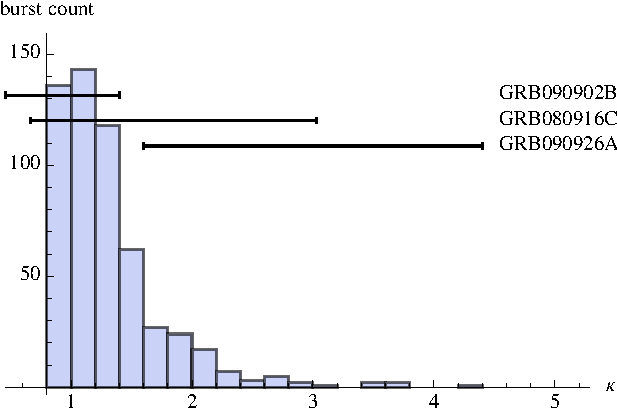
\includegraphics[width=\textwidth]{kappaDistributionHistogram}
                \label{fig:kappaDistributionHistogram}
        \end{subfigure}
        \begin{subfigure}[kappaDistributionCDF]{0.4\textwidth}
                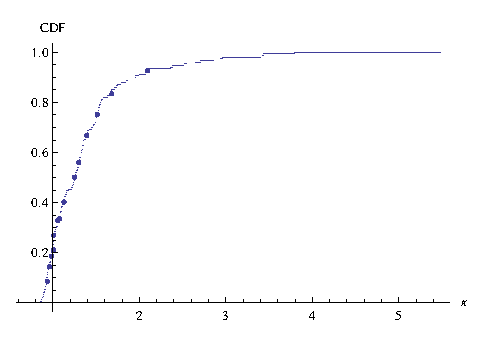
\includegraphics[width=\textwidth]{kappaDistributionCDF}
                \label{fig:kappaDistributionCDF}
        \end{subfigure}
        \caption{The histogram and the CDF of the stretching factors sample produced by our model. The sample contains $250$ points. You can see the stretching factors computed from the observations below the $\kappa$ axis (not yet implemented).}
        \label{fig:kappaDistribution}
\end{figure}

For our set of parameters, this algorithm produced a sample you can see on the figure \ref{fig:kappaDistribution}. However, the error margins of the observed stretching factors are too large to use the KS-test on them. Nevertheless, It appears that our model doesn't contradict existing observations.

\subsection{Very high energy bursts fraction}

Our final test is to calculate the fraction of the observable bursts which can be observed at the energies of GeV and above.

To do so, we need to compute the number of bursts visible in a given energy range, which is the integral over space and jet directions:
\begin{align}
b\left(\omega_1,\omega_2\right) &= \int_0^{z_\text{max}\left(\omega_1,\omega_2\right)} \dif V\left(z\right) \rho\left(z\right) \int_0^{\chi_\text{max}\left(z,\omega_1,\omega_2\right)} 2\pi \sin\chi \dif\chi \nonumber\\
&\approx 2\pi \int_0^{z_\text{max}\left(\omega_1,\omega_2\right)} \dif V\left(z\right) \rho\left(z\right) \int_0^{\chi_\text{max}\left(z,\omega_1,\omega_2\right)} \chi \dif\chi = \pi \int_0^{z_\text{max}\left(\omega_1,\omega_2\right)} \dif V\left(z\right) \rho\left(z\right) \chi^2_\text{max}\left(z,\omega_1,\omega_2\right)
\end{align}
Here $z_\text{max}\left(\omega_1,\omega_2\right)$ and $\chi_\text{max}\left(z,\omega_1,\omega_2\right)$ are the same values we used in the previous section: the maximum redshift from which a burst can be observed, and the maximum off-axis angle with which the burst at redshift $z$ can be observed.

The fraction in question is simply the ratio of these:
\begin{equation}
f\left(\omega_1,\omega_2,\omega_3\right) = \frac{b\left(\omega_2,\omega_3\right)}{b\left(\omega_1,\omega_3\right)} = \frac{\int_0^{z_\text{max}\left(\omega_2,\omega_3\right)} \dif V\left(z\right) \rho\left(z\right) \chi^2_\text{max}\left(z,\omega_2,\omega_3\right)}{\int_0^{z_\text{max}\left(\omega_1,\omega_3\right)} \dif V\left(z\right) \rho\left(z\right) \chi^2_\text{max}\left(z,\omega_1,\omega_3\right)}
\end{equation}

The ratio for our set of parameters is $f_m \approx 0.072$. The ratio computed from observations is $f_o = ...$. The binary distribution gives us the probability for it to happen:
\begin{equation}
...
\end{equation}
which means that the model fits observations in this test.

\section{Summary}

%\bibliographystyle{plain}
%\bibliography{refs}

\end{document}